\documentclass[tikz,border=6pt]{standalone}
\usepackage{amsmath,amssymb,mathtools,physics,bm,nicefrac,wasysym}
\usepackage{xcolor}

\definecolor{colone}{RGB}{180,60,60}
\definecolor{coltwo}{RGB}{60,110,180}
\definecolor{colthree}{RGB}{60,140,80}

\definecolor{accent}{HTML}{A13D2C}
\definecolor{accent2}{HTML}{2B5F6B}
\definecolor{muted}{HTML}{5A564F}
\definecolor{panel}{HTML}{F8F6F0}
\definecolor{linecol}{HTML}{D8D2C4}
\definecolor{ink}{HTML}{1E1C1A}
\definecolor{astroblue}{HTML}{1B4F72}
\definecolor{astrodark}{HTML}{17202A}
\definecolor{sunyellow}{HTML}{E8A33D}

\usetikzlibrary{calc,arrows.meta,positioning,decorations.pathreplacing,decorations.markings,angles,quotes,shapes.geometric}
\usepackage{tikz-3dplot}

\newcommand{\vecr}{\vec r}
\newcommand{\vecL}{\vec L}
\newcommand{\vecA}{\vec A}
\newcommand{\vecf}{\vec f}
\newcommand{\vecF}{\vec F}
\newcommand{\vecp}{\vec p}
\newcommand{\avg}[1]{\left\langle #1\right\rangle}
\newcommand{\vecx}{\vec x}
\newcommand{\hatn}{\hat n}
\newcommand{\rhat}{\hat r}
\newcommand{\phihat}{\hat\phi}
\newcommand{\thetahat}{\hat\theta}
\newcommand{\note}[1]{\textcolor{blue!60!black}{\textit{[#1]}}}

% Astronomical acronyms
\newcommand{\LST}{\mathrm{LST}}
\newcommand{\GST}{\mathrm{GST}}
\newcommand{\GMST}{\mathrm{GMST}}
\newcommand{\GAST}{\mathrm{GAST}}
\newcommand{\LMST}{\mathrm{LMST}}
\newcommand{\LAST}{\mathrm{LAST}}
\newcommand{\UT}{\mathrm{UT}}
\newcommand{\UTC}{\mathrm{UTC}}
\newcommand{\TAI}{\mathrm{TAI}}
\newcommand{\TT}{\mathrm{TT}}
\newcommand{\TDB}{\mathrm{TDB}}
\newcommand{\JD}{\mathrm{JD}}
\newcommand{\MJD}{\mathrm{MJD}}
\newcommand{\EoT}{\mathrm{EoT}}
\newcommand{\SNR}{\mathrm{SNR}}
\newcommand{\RON}{\mathrm{RON}}

% Helper commands for specific diagrams
\newcommand{\midlinelabel}[3]{
    \node (midlabel) at ($ (#1)!.5!(#2) $) {#3};
    \draw[stealth-] (#1) --  (midlabel);
    \draw[-stealth] (midlabel) -- (#2);
}
\newcommand{\midlinelabell}[3]{
    \node[fill = white, inner sep = 0.2pt, outer sep=3pt] (midlabel) at ($ (#1)!.5!(#2) $) {#3};
    \draw[stealth-] (#1) --  (midlabel);
    \draw[-stealth] (midlabel) -- (#2);
}
\newcommand{\midlinelabelll}[3]{
    \node[fill = white, inner sep = 0.2pt, outer sep=3pt,scale=0.6] (midlabel) at ($ (#1)!.5!(#2) $) {#3};
    \draw[stealth-] (#1) --  (midlabel);
    \draw[-stealth] (midlabel) -- (#2);
}



\begin{document}
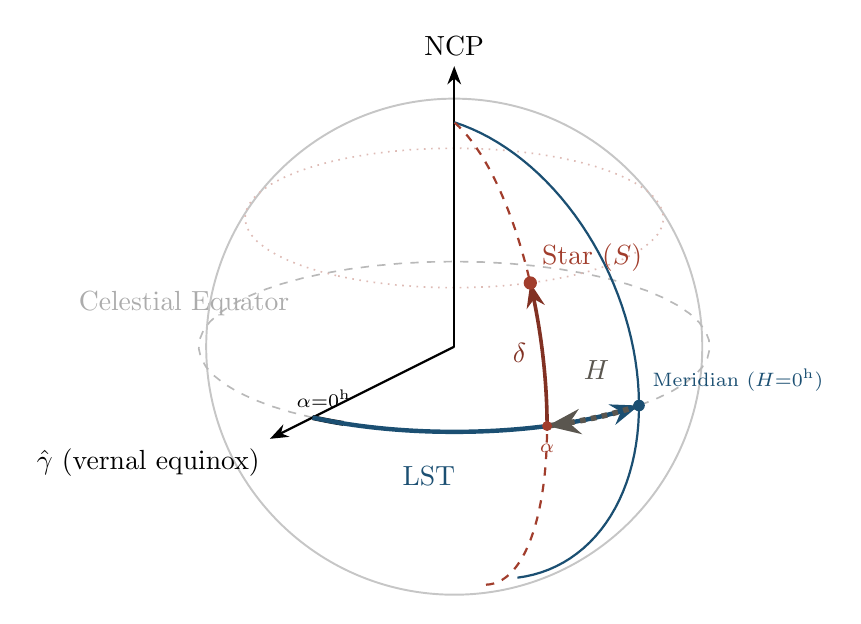
\begin{tikzpicture}[
			scale=1.5,
			x={(-0.6cm,-0.3cm)},
			y={(0.9cm,-0.2cm)},
			z={(0cm,0.95cm)},
			>=Stealth
		]
			\def\R{2.0}
			\def\LSTdeg{80}
			\def\alphaDeg{55}
			\def\deltaDeg{35}
			\pgfmathsetmacro{\Rproj}{\R*cos(\deltaDeg)}

			\coordinate (O) at (0,0,0);
			\coordinate (Xaxis) at (2.6,0,0);
			\coordinate (Zaxis) at (0,0,2.5);

			\coordinate (M) at ({\R*cos(\LSTdeg)},{\R*sin(\LSTdeg)},0);
			\coordinate (Sfoot) at ({\R*cos(\alphaDeg)},{\R*sin(\alphaDeg)},0);
			\coordinate (Star) at ({\Rproj*cos(\alphaDeg)},{\Rproj*sin(\alphaDeg)},{\R*sin(\deltaDeg)});

			% Sphere outline
			\draw[gray!45, line width=0.7pt] (0,0) circle (1.05*\R cm);

			% Celestial equator
			\draw[gray!55, dashed, line width=0.6pt] plot[domain=0:360, samples=60] ({\R*cos(\x)},{\R*sin(\x)},0);
			\node[gray!65] at ({\R*cos(250)},{\R*sin(250)},0) [below left=2pt] {Celestial Equator};

			% Star's declination (small) circle, for context -- unchanged from Figure 2.4
			\draw[accent!35, dotted, line width=0.6pt] plot[domain=0:360, samples=60] ({\Rproj*cos(\x)},{\Rproj*sin(\x)},{\R*sin(\deltaDeg)});

			% Reference axes -- vernal equinox is unchanged
			\draw[->, thick] (O) -- (Xaxis) node[below left] {$\hat\gamma$ (vernal equinox)};
			\draw[->, thick] (O) -- (Zaxis) node[above] {NCP};
			\draw[ink, line width=1.8pt] plot[domain=0:8, samples=10] ({\R*cos(\x)},{\R*sin(\x)},0);
			\node[above=1pt] at ({\R*cos(3)},{\R*sin(3)},0) {\scriptsize $\alpha{=}0^{\rm h}$};

			% Observer's meridian great circle -- now advanced past the star
			\draw[astroblue, thick] plot[domain=-70:90, samples=60]
				({\R*cos(\x)*cos(\LSTdeg)},{\R*cos(\x)*sin(\LSTdeg)},{\R*sin(\x)});

			% Star's own hour circle -- unchanged
			\draw[accent, dashed, thick] plot[domain=-70:90, samples=60]
				({\R*cos(\x)*cos(\alphaDeg)},{\R*cos(\x)*sin(\alphaDeg)},{\R*sin(\x)});

			% LST arc: full sweep from vernal equinox to the NEW (later) meridian position
			\draw[->, astroblue, line width=1.6pt] plot[domain=0:\LSTdeg, samples=40] ({\R*cos(\x)},{\R*sin(\x)},0);
			\node[astroblue] at ({\R*cos(0.35*\LSTdeg)},{\R*sin(0.35*\LSTdeg)},{-0.4}) {$\LST$};

			% H arc: the meridian has now overtaken the star; dashed overlay on the
			% shared portion of the equator, running from the meridian back to the star
			\draw[->, muted, dash pattern=on 2pt off 2pt, line width=2pt] plot[domain=\LSTdeg:\alphaDeg, samples=30] ({\R*cos(\x)},{\R*sin(\x)},0);
			\node[muted] at ({\R*cos(0.5*(\LSTdeg+\alphaDeg))},{\R*sin(0.5*(\LSTdeg+\alphaDeg))},{0.42}) {$H$};

			% delta arc (star's declination) -- unchanged
			\draw[->, accent!80!black, line width=1.3pt] plot[domain=0:\deltaDeg, samples=30]
				({\R*cos(\x)*cos(\alphaDeg)},{\R*cos(\x)*sin(\alphaDeg)},{\R*sin(\x)});
			\node[accent!80!black] at ($(Sfoot)!0.6!(Star)+(0.32,0.05,0)$) {$\delta$};

			% Points
			\fill[astroblue] (M) circle (1.4pt) node[above right=2pt] {\scriptsize Meridian ($H{=}0^{\rm h}$)};
			\fill[accent] (Sfoot) circle (1.2pt) node[below=3pt] {\scriptsize $\alpha$};
			\fill[accent] (Star) circle (1.6pt) node[above right=1pt] {Star ($S$)};
		\end{tikzpicture}
\end{document}
